\documentclass[answers]{exam}
\usepackage{marvosym}

%...TikZ & PGF
\usepackage{pgfplots}
\pgfplotsset{compat=1.11}
\tikzset{>=latex}
\usetikzlibrary{calc,math}
\usepackage{tikzsymbols}
\usepgfplotslibrary{fillbetween}
\usetikzlibrary{decorations.markings} 
\usetikzlibrary{arrows.meta} %...APP2 for arrows as objects and images
\usetikzlibrary{backgrounds} %...For shading portions of graphs
\usetikzlibrary{patterns} %...Unit 5 Problems
\usetikzlibrary{shapes.geometric} %...For drawing cylinders in Unit 2
\usepackage{makecell} %...use \thead{} to enable line skip in table headers
\tikzset{
    mark position/.style args={#1(#2)}{
        postaction={
            decorate,
            decoration={
                markings,
                mark=at position #1 with \coordinate (#2);
            }
        }
    }
} %...See https://tex.stackexchange.com/questions/43960/define-node-at-relative-coordinates-of-draw-plot

\tikzset{
    declare function = {trajectoryequation10(\x,\vi,\thetai)= tan(\thetai)*\x - 10*\x^2/(2*(\vi*cos(\thetai))^2);},
    declare function = {trajectoryequation(\x,\vi,\thetai)= tan(\thetai)*\x - 9.8*\x^2/(2*(\vi*cos(\thetai))^2);},
    declare function = {patheq(\x,\yi,\vi,\thetai)= \yi + tan(\thetai)*\x - 9.8*\x^2/(2*(\vi*cos(\thetai))^2);},
    declare function = {patheqten(\x,\yi,\vi,\thetai)= \yi + tan(\thetai)*\x - 10*\x^2/(2*(\vi*cos(\thetai))^2);} %like patheq but with gravity = 10
}

%...siunitx
\usepackage{siunitx}
\DeclareSIUnit{\nothing}{\relax}
\def\mymu{\SI{}{\micro\nothing} }
\DeclareSIUnit\mmHg{mmHg}
\DeclareSIUnit{\mile}{mi}
%...NOTE: "The product symbol between the number and unit is set using the quantity-product option."

%...Other
\usepackage{amsthm}
\usepackage{amsmath}
\usepackage{amssymb}
\usepackage{cancel}
\usepackage{subcaption}
\usepackage{dashrule}
\usepackage{enumitem}
\usepackage{fontawesome}
\usepackage{multicol}
\usepackage{glossaries}
%\numberwithin{equation}{section}
\numberwithin{figure}{section}
\usepackage{float}
\usepackage{twemojis} %...twitter emojis
\usepackage{utfsym}
\usepackage{linearb} %...For \BPwheel in Unit 8
\newcommand{\R}{\mathbb{R}} %...real number symbol
\usepackage{graphicx}
\graphicspath{ {../Figures/} }
\usepackage{hyperref}
\hypersetup{colorlinks=true,
    linkcolor=blue,
    filecolor=magenta,
    urlcolor=cyan,}
\urlstyle{same}
\newcommand{\hdashline}{{\hdashrule{\textwidth}{0.5pt}{0.8mm}}}
\newcommand{\hgraydashline}{{\color{lightgray} \hdashrule{0.99\textwidth}{1pt}{0.8mm}}}

%...Miscellaneous user-defined symbols
\newcommand{\fnet}{F_{\text{net}}} %...For net force
\newcommand{\bvec}[1]{\vec{\mathbf{#1}}} %...bold vector
\newcommand{\bhat}[1]{\,\hat{\mathbf{#1}}} %...bold hat vector
\newcommand{\que}{\mathord{?}}  %...Question mark symbol in equation env
%...Define thick horizontal rule for examples:
\newcommand{\hhrule}{\hrule\hrule}
\let\oldtexttt\texttt% Store \texttt
\renewcommand{\texttt}[2][black]{\textcolor{#1}{\ttfamily #2}}% 

%...For use in the exam document class
\newif\ifprintmetasolutions


%...Decreases space above and below align and gather enironment
\makeatletter
\g@addto@macro\normalsize{%
  \setlength\abovedisplayskip{-3pt}
  \setlength\belowdisplayskip{6pt} 
}
\makeatother





\usepackage[margin=1in]{geometry}
\usepackage[figurewithin=none]{caption}
\usepackage{exam-randomizechoices}
\setrandomizerseed{1}

\CorrectChoiceEmphasis{\color{red}\bfseries}
\renewcommand{\solutiontitle}{\noindent\textbf{\textcolor{red}{Solution:}}\enspace}

\usepackage{OutilsGeomTikz}
\usepackage{utfsym} %...Symbols in Unit 7 Problems
\usepackage{tabu} %...Symbols in Unit 7 Problems

%...For use in Unit 2            %    
\setlength{\columnsep}{2cm}      %
\setlength{\columnseprule}{1pt}  %
\usepackage[none]{hyphenat}      %
%%%%%%%%%%%%%%%%%%%%%%%%%%%%%%%%%

%...For use in Unit 11 on Waves:
\pgfdeclarehorizontalshading{visiblelight}{50bp}{  %
color(0.00000000000000bp)=(red);                   %
color(8.33333333333333bp)=(orange);                %
color(16.66666666666670bp)=(yellow);               %
color(25.00000000000000bp)=(green);                %
color(33.33333333333330bp)=(cyan);                 %
color(41.66666666666670bp)=(blue);                 %
color(50.00000000000000bp)=(violet)                %
}                                                  %

\newcommand{\checkbox}[1]{%
  \ifnum#1=1
    \makebox[0pt][l]{\raisebox{0.15ex}{\hspace{0.1em}\Large$\checkmark$}}%
  \fi
  $\square$%
}
%%%%%%%%%%%%%%%%%%%%%%%%%%%%%%%%%%%%%%%%%%%%%%%%%%%%

%...If using circuitikz package:
% \ctikzset{bipoles/battery1/height=0.5}
% \ctikzset{bipoles/battery1/width=0.25}
% \ctikzset{bipoles/resistor/height=0.15}
% \ctikzset{bipoles/resistor/width=0.4}
\usepackage{circuitikz}
\ctikzset{bipoles/battery1/height=0.5}
\ctikzset{bipoles/battery1/width=0.25}
\ctikzset{bipoles/battery/height=0.4}
\ctikzset{bipoles/battery/width=0.2}
\ctikzset{bipoles/resistor/height=0.17}
\ctikzset{bipoles/resistor/width=0.38}
\ctikzset{bipoles/capacitor/width=0.1}
\ctikzset{bipoles/capacitor/height=0.4}
\ctikzset{bipoles/cuteswitch/thickness=0.3,bipoles/cuteswitch/shape=circ}
\ctikzset{bipoles/bulb/height=0.4,bipoles/bulb/width=0.4}


\setrandomizerseed{1}
\bracketedpoints

\newif\ifversionKlevel

\versionKleveltrue

\header{Physics\\Review on Unit 9: Conservation of Charge}{}{Name:\enspace\makebox[5cm]{\hrulefill}}

\ifversionKlevel
    \header{Physics\\Review on Unit 9: Conservation of Charge}{}{Name:\enspace\makebox[5cm]{\hrulefill}}
\fi

\begin{document}

% \section*{Electrostatics Quiz}

\begin{questions}

\question
The SI unit of charge is the \fillin[Coulomb][3cm].

% \begin{randomizechoices}
%     \choice Newton
%     \choice Ampere
%     \choice Joule
%     \correctchoice Coulomb
% \end{randomizechoices}

\question
Which of the charges shown in the image below is positive? \fillin[A].

\begin{center}
    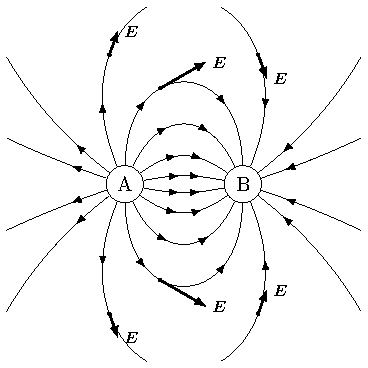
\includegraphics[width=5cm]{documents/figures/electric-field-lines-1.pdf}
\end{center}

% \begin{randomizechoices}[norandomize]
%     \correctchoice A
%     \choice B
%     \choice Both
%     \choice Neither
% \end{randomizechoices}

\question
Which statement best describes the charge of the slab below?

\bgroup
\begin{center}
\large
\begin{tikzpicture}[x=3.5mm,y=3.5mm]
    \draw (0,1) rectangle (7,5);
    \node at (1,4) {\faPlusCircle};
    \node at (2,3) {\faMinusCircle};
    \node at (3,2) {\faPlusCircle};
    \node at (4.5,2) {\faMinusCircle};
    \node at (3,4) {\faPlusCircle};
    \node at (4,3) {\faPlusCircle};
    \node at (6,2) {\faPlusCircle};
\end{tikzpicture}
\end{center}
\egroup

\begin{randomizechoices}[keeplast]
    \correctchoice positively charged
    \choice negatively charged
    \choice neutral
    \choice There is not enough information to tell .
\end{randomizechoices}

\question
According to Coulomb’s Law, if you increase the distance between two objects by a factor of 2, the electrical force between them will

\begin{randomizechoices}
    \choice decrease by a factor of 2.
    \choice increase by a factor of 2.
    \correctchoice decrease by a factor of 4.
    \choice increase by a factor of 4.
\end{randomizechoices}

% \question
% \phantom{.}

\question
When does a repelling force occur between two charged objects? 

\ifprintanswers
{\color{red}
When the objects have the same charge (e.g. both positive or both negative).
}
\else
\fillwithlines{1.5cm}
\fi
% \begin{randomizechoices}
%     \correctchoice charges are of like signs.
%     \choice charges are of equal magnitude.
%     \choice charges are of opposite signs.
%     \choice charges are of unequal magnitude.
% \end{randomizechoices}

\question
Which point charge in the image below has the strongest electric field? \fillin[C]

\begin{center}
\begin{tikzpicture}[x=1.5cm,y=1.5cm]
    \foreach \x in {0,45,...,315}{
        \draw[->,thick,rotate=\x] (0,0) -- (1,0);
    }
    \draw[fill=white] (0,0) circle (3mm) node {A};
\end{tikzpicture}
\hspace{1cm}
\begin{tikzpicture}[x=1.5cm,y=1.5cm]
    \foreach \x in {0,22.5,...,337.5}{
        \draw[->,thick,rotate=\x] (0,0) -- (1,0);
    }
    \draw[fill=white] (0,0) circle (3mm) node {B};
\end{tikzpicture}
\hspace{1cm}
\begin{tikzpicture}[x=1.5cm,y=1.5cm]
    \foreach \x in {0,11.25,...,348.75}{
        \draw[->,thick,rotate=\x] (0,0) -- (1,0);
    }
    \draw[fill=white] (0,0) circle (3mm) node {C};
\end{tikzpicture}
\end{center}

% \begin{randomizechoices}[norandomize]
%     \choice A
%     \choice B
%     \correctchoice C
%     \choice Cannot determine.
% \end{randomizechoices}

\question
What particle(s) in the nucleus of an atom has/have an electric charge? \fillin[protons only]

% \begin{randomizechoices}[norandomize]
%     \choice Electrons
%     \correctchoice Protons
%     \choice Neutrons
%     \choice A \& B
%     \choice None of the above
% \end{randomizechoices}

\question
Describe how an object becomes negatively charged.

\ifprintanswers
{\color{red}
By gaining electrons. For example, when a balloon is rubbed against a shirt, friction strips electrons away from the shirt and to the balloon.}
\else
\fillwithlines{1.3cm}
\fi

% \begin{randomizechoices}
%     \choice By losing protons
%     \correctchoice By gaining electrons
%     \choice By gaining neutrons
%     \choice By losing neutrons
% \end{randomizechoices}

\question
What is the difference between charging by conduction and charging by induction?

\ifprintanswers
{\color{red}
In induction the objects don’t touch, but in conduction they do.
}
\else
\fillwithlines{1.3cm}
\fi

% \begin{randomizechoices}
%     \choice In conduction the objects don’t touch, but in induction they do.
%     \correctchoice In induction the objects don’t touch, but in conduction they do.
%     \choice Charges separate on the same side of one object in conduction.
%     \choice Charges do not move in induction but they do in conduction .
% \end{randomizechoices}

\question
While taking his clothes out of the dryer, Charles finds a sock clinging to his sweater. What is the best explanation for this common phenomenon? 

\ifprintanswers
{\color{red}
In the dryer, either the sock or the sweater gained electrons while the other item lost electrons.
}
\else
\fillwithlines{1.3cm}
\fi

% \begin{randomizechoices}[keeplast]
%     \choice In the dryer, both the sock and the sweater lost electrons.
%     \choice In the dryer, both the sock and the sweater gained electrons.
%     \correctchoice In the dryer, either the sock or the sweater gained electrons while the other item lost electrons
%     \choice The cause of static cling is an unsolved scientific mystery.
% \end{randomizechoices}

\question
Pith Ball A is known to have a positive charge.  Based on the experiments in the diagram below, determine the charge of Pith Balls B and C.

\begin{center}
\begin{tikzpicture}
    \draw (0,0) -- (3,0);
    \draw (0.2,0) -- (1.1,-1);
    \draw (2.8,0) -- (1.9,-1);
    \draw[fill=white] (1.1,-1) circle (3mm) node {A};
    \draw[fill=white] (1.9,-1) circle (3mm) node {B};
\end{tikzpicture}
\hspace{1cm}
\begin{tikzpicture}
    \draw (0,0) -- (3,0);
    \draw (1.4,0) -- (0.5,-1);
    \draw (1.6,0) -- (2.5,-1);
    \draw[fill=white] (0.5,-1) circle (3mm) node {C};
    \draw[fill=white] (2.5,-1) circle (3mm) node {B};
\end{tikzpicture}
\end{center}

\begin{randomizechoices}
    \correctchoice Both B and C are negative.
    \choice B is positive and C is negative.
    \choice Both B and C are positive.
    \choice B is negative and C is positive.
\end{randomizechoices}

\question
Consider an isolated system consisting of two charges only. In the figure below, $Q_1$ is positive and $Q_2$ is negative.  How are the gravitational force and electrostatic force acting on $Q_1$ related to each other?

% \begin{center}
% \fbox{
\begin{minipage}{9cm}
\begin{randomizechoices}
    \correctchoice They are going in the same direction.
    \choice They are perpendicular.
    \choice The are going in opposite directions.
    \choice They are both 0.
\end{randomizechoices}
\end{minipage}
% }
%
% \fbox{
\begin{minipage}{3cm}
\centering
\begin{tikzpicture}
    \draw (0,2) -- (0,0) -- (2,0);
    \fill (0,1.5) circle (2pt) node[right=2pt] {$Q_1$};
    \fill (1.5,0) circle (2pt) node[below=2pt] {$Q_2$};
\end{tikzpicture}    
\end{minipage}
% }
% \end{center}




\question
Two particles with charges of $+4q$ and $-2q$ are a distance $3r$ apart. Which of the following is an expression for the magnitude of the electric force between them?

\begin{randomizeoneparchoices}
    \correctchoice $\displaystyle \frac{8kq^2}{9r^2}$
    \choice $\displaystyle \frac{8kq^2}{3r^2}$
    \choice $\displaystyle \frac{8kq^2}{r^2}$
    \choice $\displaystyle \frac{kq^2}{9r^2}$
\end{randomizeoneparchoices}

\question
A \SI{5}{\micro\coulomb} charge and a \SI{12}{\micro\coulomb} charge are located \SI{0.25}{m} apart. Calculate the electrostatic force acting between them.

\begin{solutionorbox}[4cm]
The electric force is given by Coulomb's law:

\begin{equation*}
    F = \frac{kq_1q_2}{r^2} = \frac{\left(\SI{9e9}{N\cdot m^2/C^2}\right)(\SI{5e-6}{C})(\SI{12e-6}{C})}{(\SI{0.25}{m})^2} = \SI{8.64}{N}
\end{equation*}
\end{solutionorbox}

% \end{questions}

\clearpage

% \section*{Circuits Quiz}

% \begin{questions}
\question
Electrons are the mobile charge carriers in an electric circuit.

\begin{randomizechoices}[norandomize]
    \correctchoice True
    \choice False
\end{randomizechoices}

\question
Name all the components that are present in this circuit diagram below.
\bigskip

\fillin[a battery, 2 resistors, and a swtich][15cm]

\begin{center}
\begin{tikzpicture}[x=1.5cm,y=1.5cm]
    \draw (0,2) to[battery1] (0,1) to[R] (0,0) -- (1,0) to[R] (1,2) -- (0,2);
    \draw (1,2) -- (2,2) to[cute open switch] (2,0) -- (1,0);
\end{tikzpicture}
\end{center}

% \begin{randomizechoices}
%     \choice Bulb, switch, battery
%     \choice Variable resistor, diode, battery
%     \correctchoice Switch, resistors, battery
%     \choice Resistor, switch, capacitor
% \end{randomizechoices}

\question
Which of the following household devices uses the most power when plugged into a \SI{120}{V} outlet?

\begin{solution}
Power is the product of current and voltage: $P = IV$. Therefore, the device with the largest current will use the most power.
\end{solution}

\begin{randomizechoices}
    \choice A laptop running with \SI{1.0}{A}
    \choice A video game player and TV that use \SI{3.2}{A} total
    \correctchoice A microwave oven running with \SI{4.2}{A}
    \choice A cell phone charger that uses \SI{0.1}{A}
\end{randomizechoices}

\question
The flow of electricity in a circuit requires a \fillin[complete or closed][5cm] path.

% \begin{randomizechoices}
%     \correctchoice complete path
%     \choice complex circuit
%     \choice insulated current
%     \choice incomplete path
% \end{randomizechoices}

\question
If a light bulb uses a current of \SI{4.0}{A} and has a resistance of \SI{3.0}{\ohm}, what is the voltage drop across it?

\fillin[\SI{12}{V}]

% \begin{randomizechoices}
%     \correctchoice \SI{12}{V}
%     \choice \SI{1.0}{V}
%     \choice \SI{1.3}{V}
%     \choice \SI{0.75}{V}
% \end{randomizechoices}

\question
Identify the symbol shown in the image below. \fillin[battery]

\begin{center}
\begin{tikzpicture}
    \draw (1,0) to[battery1] (0,0);
\end{tikzpicture}
\end{center}

% \begin{randomizechoices}
%     \choice Wires
%     \choice Switch
%     \choice Light bulb
%     \correctchoice Battery 
% \end{randomizechoices}

\question
What physical quantity is related to the electron flow in a circuit? \fillin[current]

% \begin{randomizechoices}
%     \choice Power
%     \choice Potential difference
%     \choice Conductor
%     \correctchoice Current
% \end{randomizechoices}

\question
In this circuit, which branch has more current flowing through it?

\ifprintanswers
{\color{red}
The branch with the \SI{2}{\ohm} resistor.
}
\else
\fillwithlines{1cm}
\fi

\begin{center}
\begin{tikzpicture}[x=1.5cm,y=1.8cm]
    \draw (0,1) to[battery1,l_={\SI{12}{V}}] (0,0) -- (2,0) to[R,l_={\SI{6}{\ohm}}] (2,1) -- (0,1);
    \draw (1,1) to[R={\SI{2}{\ohm}}] (1,0);
\end{tikzpicture}
\end{center}

% \begin{randomizechoices}[keeplast]
%     \correctchoice The branch with the \SI{2}{\ohm} resistor.
%     \choice The branch with the \SI{6}{\ohm} resistor.
%     \choice Both branches have the same current.
%     \choice There is not enough information to tell.
% \end{randomizechoices}

\question
As the number of resistors increases in series across a battery, what happens to the voltage drop across each resistor?

\fillin[Voltage drop decreases.][14cm]

% \begin{randomizechoices}[keeplast]
%     \correctchoice decreases.
%     \choice stays the same.
%     \choice increases.
%     \choice There is not enough information.
% \end{randomizechoices}

\question
The electric current in a circuit will increase as the electric potential across a circuit is increased.

\begin{randomizechoices}[norandomize]
    \correctchoice True 
    \choice False
\end{randomizechoices}

\question
What is the current through a \SI{11}{V} bulb with a power of \SI{99}{W}? \fillin[\SI{9.0}{A}]

% \begin{randomizechoices}
%     \choice \SI{60}{A}
%     \choice \SI{99}{A}
%     \correctchoice \SI{9.0}{A}
%     \choice \SI{88}{A}
% \end{randomizechoices}

\question
If the total resistance of the circuit shown is \SI{15}{\ohm}, what is the value of resistor $R$?

\begin{center}
\begin{tikzpicture}[x=1.5cm,y=1.5cm]
    \draw (0,0) to[R,l_={$R$}] (2,0) to[R,l_={\SI{2}{\ohm}}] (2,1) to[R,l_={\SI{1}{\ohm}}] (1,1) to[battery] (0,1) to[R,l_={\SI{3}{\ohm}}] (0,0);
\end{tikzpicture}
\end{center}

\begin{solutionorbox}[3.0cm]
In series, the total resistance is given by

\begin{equation*}
    R_\mathrm{eq} = R_1 + R_2 + R_3 + R
\end{equation*}

We know that $R_\mathrm{eq} = \SI{15}{\ohm}$. So,

\begin{equation*}
    \SI{15}{\ohm} = \SI{1}{\ohm} + \SI{2}{\ohm} + \SI{3}{\ohm} + R
\end{equation*}

which simplifies to

\begin{equation*}
    \SI{15}{\ohm} = \SI{6}{\ohm} + R
\end{equation*}

Therefore, solving for $R$, we get

\begin{equation*}
    R = \SI{15}{\ohm} - \SI{6}{\ohm} = \boxed{\SI{9}{\ohm}}
\end{equation*}
\end{solutionorbox}

% \begin{randomizechoices}
%     \correctchoice \SI{9}{\ohm}
%     \choice \SI{12}{\ohm}
%     \choice \SI{18}{\ohm}
%     \choice \SI{6}{\ohm}
% \end{randomizechoices}

\question
What is the power of a \SI{10}{V} bulb with \SI{5}{A} through it?

\begin{solutionorbox}[2.5cm]
Power is

\begin{equation*}
    P = IV = (\SI{5}{A})(\SI{10}{V}) = \boxed{\SI{50}{W}} 
\end{equation*}
\end{solutionorbox}

% \begin{randomizechoices}
%     \choice \SI{2}{V}
%     \choice \SI{2}{W}
%     \choice \SI{50}{A}
%     \correctchoice \SI{50}{W}
% \end{randomizechoices}

\question
What is the total resistance of the circuit?

\begin{center}
\begin{tikzpicture}[x=1.5cm,y=1.5cm]
    \draw (0,1) to[battery] (0,0) to[R,l_={\SI{25}{\ohm}}] (1,0) to[R,l_={\SI{100}{\ohm}}] (1,1) to[R,l_={\SI{75}{\ohm}}] (0,1);
\end{tikzpicture}
\end{center}

\begin{solutionorbox}[2.0cm]
In series, total resistance is the sum of resistances:

\begin{align*}
    R_\mathrm{eq} &= R_1 + R_2 + R_3 \\[1ex]
    &= \SI{75}{\ohm} + \SI{100}{\ohm} + \SI{25}{\ohm} \\[1ex]
    &= \boxed{\SI{200}{\ohm}}
\end{align*}
\end{solutionorbox}

% \begin{randomizechoices}
%     \choice \SI{15.8}{\ohm}
%     \correctchoice \SI{200}{\ohm}
%     \choice \SI{0.63}{\ohm}
%     \choice \SI{100}{\ohm}
% \end{randomizechoices}

\question
The diagram below represents part of an electric circuit containing three parallel resistors. What is the equivalent resistance of this part of the circuit?

\begin{minipage}{6cm}
\centering
\begin{tikzpicture}[x=1.5cm,y=1.2cm]
    \draw (0,0) to[R={\SI{12}{\ohm}}] (1,0) -- (1,2) to[R,l_={\SI{3.0}{\ohm}}] (0,2) -- (0,0);
    \draw[shift={(-0.5,1)}] (0,0) to[R={\SI{4.0}{\ohm}}] (2,0);
\end{tikzpicture}
\end{minipage}%
\fbox{
\begin{minipage}{9cm}
\ifprintanswers
\color{red}
\else
\color{white}
\fi

\vspace{1em}

\begin{align*}
    R_\mathrm{eq} &= \left(\frac{1}{R_1} + \frac{1}{R_2} + \frac{1}{R_3}\right)^{-1} \\[1ex]
    &= \left(\frac{1}{\SI{3.0}{\ohm}} + \frac{1}{\SI{4.0}{\ohm}} + \frac{1}{\SI{12}{\ohm}}\right)^{-1} \\[1ex]
    &= \boxed{\SI{1.5}{\ohm}}
\end{align*}

\vspace{1em}
\end{minipage}
}


% \begin{center}

% \end{center}



\end{questions}

\end{document}
